\documentclass{beamer}

\usetheme{Boadilla}

%\includeonlyframes{current}

\usepackage{times}
\usefonttheme{structurebold}
\usepackage{listings}
\usepackage{ragged2e}

\usepackage{pgf}
\usepackage{tikz}
\usepackage{alltt}
\usepackage[normalem]{ulem}
\usetikzlibrary{arrows}
\usetikzlibrary{automata}
\usetikzlibrary{shapes}
\usepackage{amsmath,amssymb}
\usepackage{rotating}
\usepackage{ulem}
\usepackage{listings}
\usepackage{enumerate}
\usepackage{tikz}
\tikzset{
  every overlay node/.style={
    draw=black,fill=white,rounded corners,anchor=north west,
  },
}
\def\tikzoverlay{%
   \tikz[baseline,overlay]\node[every overlay node]
}%

%\setbeamercovered{dynamic}
\setbeamertemplate{footline}[page number]{}
\setbeamertemplate{navigation symbols}{}
\usefonttheme{structurebold}

\title{Software Testing, Quality Assurance \& Maintenance---Lecture 10}
\author{Patrick Lam\\University of Waterloo}
\date{January 26, 2015}

\colorlet{redshaded}{red!25!bg}
\colorlet{shaded}{black!25!bg}
\colorlet{shadedshaded}{black!10!bg}
\colorlet{blackshaded}{black!40!bg}

\colorlet{darkred}{red!80!black}
\colorlet{darkblue}{blue!80!black}
\colorlet{darkgreen}{green!80!black}

\newcommand{\rot}[1]{\rotatebox{90}{\mbox{#1}}}
\newcommand{\gray}[1]{\mbox{#1}}

\newenvironment{changemargin}[1]{% 
  \begin{list}{}{% 
    \setlength{\topsep}{0pt}% 
    \setlength{\leftmargin}{#1}% 
    \setlength{\rightmargin}{1em}
    \setlength{\listparindent}{\parindent}% 
    \setlength{\itemindent}{\parindent}% 
    \setlength{\parsep}{\parskip}% 
  }% 
  \item[]}{\end{list}}


\lstset{ %
language=C++,
basicstyle=\ttfamily,commentstyle=\scriptsize\itshape,showstringspaces=false,breaklines=true}

\begin{document}

\begin{frame}
  \titlepage
\end{frame}

\begin{frame}
  \frametitle{Course roadmap}

  \begin{changemargin}{2cm}
  \begin{itemize}
  \item $\checkmark$ Introduction (faults etc)
  \item $\checkmark$ Graph coverage
  \item $\Box$ \alert{Testing Concurrent Programs}
  \end{itemize}
  \end{changemargin}
\end{frame}

\begin{frame}
\frametitle{Concurrency In Your Curriculum}
\begin{changemargin}{2cm}
  SE350 (OS): \\
  \hspace*{2em} first exposure to multiprocessing\\[1em]
  CS343 (Concurrency): \\
  \hspace*{2em} (obvious) \\[1em]
  ECE459 (4B, P4P): \\
  \hspace*{2em} learn more about leveraging parallelism!
\end{changemargin}
\end{frame}

\begin{frame}
\frametitle{Context: Multicores, everywhere, today}
  \begin{changemargin}{2cm}
    For past 10 years, chips not getting faster.\\[1em]
    Solution:
    \begin{center}
    
\includegraphics[width=2em]{L10/centrino-duo}
    
\includegraphics[width=2em]{L10/core-2-duo}
    
\includegraphics[width=2em]{L10/core-2-quad}
    \end{center}

    Multicores!\\[2em]
    \begin{tabbing}
    Today:~~\=if you want performance, \\
    \>then you need parallelism.
    \end{tabbing}
    ~\\[0.5em]
    Implication: concurrency bugs will bite you. 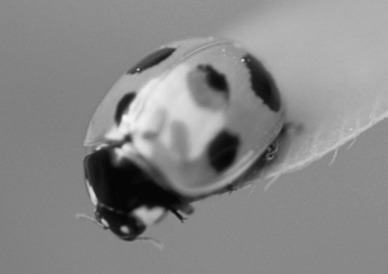
\includegraphics[width=2em]{L10/ladybug}
  \end{changemargin}

\end{frame}

\begin{frame}
  \begin{changemargin}{0cm}
    \begin{center}
    \begin{minipage}{.8\textwidth}
    {\Large \justifying
      ``More often than not, printing a page on my dual-G5 crashes the application. The funny thing is, printing almost never crashes on my (single-core) G4 PowerBook.''\\
    }
    \end{minipage}
    \end{center}~\\[1em]
    \hfill \scriptsize \url{http://archive.oreilly.com/pub/post/dreaded_concurrency.html}
  \end{changemargin}
\end{frame}

\begin{frame}
  \frametitle{Race Conditions}
  \begin{center}
    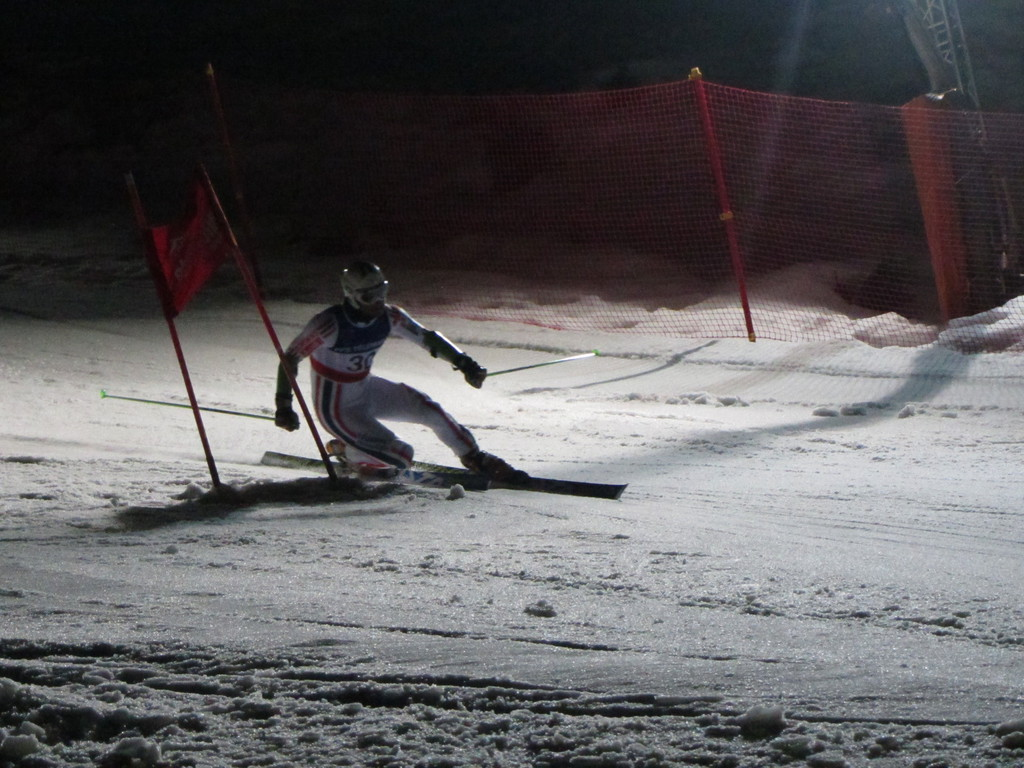
\includegraphics[width=.8\textwidth]{L10/5482_racer}
    
    \hfill credit: me
  \end{center}
\end{frame}

\begin{frame}
  \frametitle{Alas!}
  \scriptsize
  \begin{changemargin}{2cm}
    \lstinputlisting{live-coding/L10/race.C}
  \end{changemargin}
\end{frame}

\begin{frame}[fragile]
  \frametitle{Racy Output}
  \begin{changemargin}{2cm}
\begin{verbatim}
plam@polya /tmp> ./a.out
2⏎
plam@polya /tmp> ./a.out
2⏎
plam@polya /tmp> ./a.out
1⏎
plam@polya /tmp> ./a.out
1⏎
plam@polya /tmp> ./a.out
2⏎
plam@polya /tmp> ./a.out
2⏎
\end{verbatim}
  \end{changemargin}
\end{frame}

%%%%%%%%%%%%%%%%%%%%%%%%%%%%%%%%%%%%%%%%%%%%%%%%%%%%%%%%%%%%%%%%%%%%%%%%%%%%%%%%
\begin{frame}
  \frametitle{Race Conditions [from ECE459 slides]}

  \begin{changemargin}{2.5cm}
  \begin{itemize}
    \item A race occurs when you have two concurrent accesses to the
      same memory location, at least one of which is a {\bf write}.
  \end{itemize}~\\

   When there's a race, the final state may not be the same as
      running one access to completion and then the other.\\[1em]
   Race conditions arise between variables which
      are shared between threads.
  \end{changemargin}

\end{frame}
%%%%%%%%%%%%%%%%%%%%%%%%%%%%%%%%%%%%%%%%%%%%%%%%%%%%%%%%%%%%%%%%%%%%%%%%%%%%%%%%

\begin{frame}
  \frametitle{Tools for Detecting Races}
  \begin{changemargin}{2cm}
    \begin{itemize}
    \item Helgrind (part of Valgrind)
    \item lockdep (Linux kernel)
    \item Thread Analyzer (Oracle Solaris Studio)
    \item Thread Analyzer (Coverity)
    \item Intel Inspector XE 2011 \\
      \hspace*{2em}(formerly Intel Thread Checker)
    \item [and more]
    \end{itemize}
  \end{changemargin}
\end{frame}

\begin{frame}[fragile]
  \frametitle{Helgrind Example}
    \scriptsize
\begin{verbatim}
plam@polya /tmp> g++ -std=c++11 race.C -g -pthread -o race
plam@polya /tmp> valgrind --tool=helgrind ./race
[...]
==6486== Possible data race during read of size 4 at 0x603E1C by thread #3
==6486== Locks held: none
==6486==    at 0x400EA1: func() (race.C:8)
==6486==    by 0x402254: void std::_Bind_simple<void (*())()>::_M_invoke<>(std::_Index_tuple<>) (functional:1732)
==6486==    by 0x4021AE: std::_Bind_simple<void (*())()>::operator()() (functional:1720)
==6486==    by 0x402147: std::thread::_Impl<std::_Bind_simple<void (*())()> >::_M_run() (thread:115)
==6486==    by 0x4EF196F: ??? (in /usr/lib/x86_64-linux-gnu/libstdc++.so.6.0.20)
==6486==    by 0x4C2F056: mythread_wrapper (hg_intercepts.c:234)
==6486==    by 0x56650A3: start_thread (pthread_create.c:309)
==6486==    by 0x595FCCC: clone (clone.S:111)
==6486== 
==6486== This conflicts with a previous write of size 4 by thread #2
==6486== Locks held: none
==6486==    at 0x400EB1: func() (race.C:10)
==6486==    by 0x402254: void std::_Bind_simple<void (*())()>::_M_invoke<>(std::_Index_tuple<>) (functional:1732)
==6486==    by 0x4021AE: std::_Bind_simple<void (*())()>::operator()() (functional:1720)
==6486==    by 0x402147: std::thread::_Impl<std::_Bind_simple<void (*())()> >::_M_run() (thread:115)
==6486==    by 0x4EF196F: ??? (in /usr/lib/x86_64-linux-gnu/libstdc++.so.6.0.20)
==6486==    by 0x4C2F056: mythread_wrapper (hg_intercepts.c:234)
==6486==    by 0x56650A3: start_thread (pthread_create.c:309)
==6486==    by 0x595FCCC: clone (clone.S:111)
==6486==  Address 0x603e1c is 0 bytes inside data symbol "counter"
\end{verbatim}
\end{frame}

\begin{frame}
  \frametitle{Eliminating Races Ain't Enough}
  \begin{changemargin}{2cm}
    Race-freedom required by specification,\\
    but doesn't guarantee bug-freedom.\\[1em]

    {\scriptsize
      \lstinputlisting{live-coding/L10/still-race.C}
      }
  \end{changemargin}
\end{frame}

\begin{frame}
  \frametitle{Testing Race-Free Programs}
  \begin{changemargin}{2cm}
    \Large
    Race free? That don't impress me much. Now what?
    \begin{itemize}
    \item run your code multiple times
    \item add noise\\ \hspace*{2em} (sleep, more system load, etc)
    \item Helgrind and friends
    \item force scheduling\\ \hspace*{2em} (e.g. Java PathFinder)
    \item static approaches: \\ \hspace*{2em} lock-set, happens-before,\\
      \hspace*{2em} state-of-the-art techniques
    \end{itemize}
    
  \end{changemargin}
\end{frame}

\begin{frame}
  \frametitle{Reentrant/recursive Locks}
  \begin{changemargin}{2cm}
    What happens if you have two requests for a POSIX/C++11 lock?\\[1em]
    \only<2->{Different threads: \\ \hspace*{1em} second thread waits for first to unlock.\\[1em]}
    \only<3->{Same thread: \\ \hspace*{1em} first thread waits for first to unlock\ldots forever!\\[1em]

      However, you can use \emph{recursive} locks.}
  \end{changemargin}
\end{frame}
      
\begin{frame}[fragile]
  \frametitle{Reentrant/recursive Locks}
  \begin{changemargin}{2cm}
    Each lock knows how many times its owner has locked it.\\[1em]
    Must unlock same number of times to liberate.\\[2em]
    Java locks work this way, e.g.
    \begin{lstlisting}[language=Java]
class SynchronizedIsRecursive {
  int x;

  synchronized void f() {
    x--;
    g(); // does not hang!
  }

  synchronized void g() {
    x++;
  }
}
    \end{lstlisting}
  \end{changemargin}
\end{frame}

      
\begin{frame}[fragile]
  \frametitle{Java {\tt ReentrantLock}s}
  \begin{changemargin}{2cm}
    Although every Java object is a lock,\\ {\tt ReentrantLocks} are more special.\\[1em]

    \begin{itemize}
    \item can explicitly {\tt lock()} \& {\tt unlock()} them,
    \item or even {\tt trylock()}!
    \end{itemize}
~\\[1em]
    \alert{CAVEAT:} not cool to hog the lock---do this
    \begin{lstlisting}[language=Java]
Lock lock = new ReentrantLock();
lock.lock();
try {
  // you got the lock! workworkwork
} finally {
  // might have thrown an exception
  lock.unlock();
}
    \end{lstlisting}
  \end{changemargin}
  
\end{frame}

\part{Bad Lock Usage}
\begin{frame}
  \partpage
\end{frame}

\begin{frame}
  \begin{changemargin}{2cm}\small
    Reference: \\[1em]
    Dawson Engler, David Yu Chen, Seth Hallem, Andy Chou, Benjamin Chelf.\\
  ``Bugs as Deviant Behavior: a general approach to inferring errors in system code.''\\
  ACM Symposium on Operating Systems Principles, 2001.
  \end{changemargin}
\end{frame}

\begin{frame}[fragile]
  \frametitle{\ldots nice try}
    \begin{lstlisting}[language=C,commentstyle={\color{red}\bf}]
/* 2.4.0:drivers/sound/cmpci.c:cm_midi_release: */
lock_kernel(); // [PL: GRAB THE LOCK]
if (file->f_mode & FMODE_WRITE) {
  add_wait_queue(&s->midi.owait, &wait);
  ...
  if (file->f_flags & O_NONBLOCK) {
    remove_wait_queue(&s->midi.owait, &wait);
    set_current_state(TASK_RUNNING);
    return -EBUSY; // [PL: OH NOES!!1]
  }
  ...
}
unlock_kernel();
    \end{lstlisting}
    \begin{changemargin}{1cm}
      \Large
      Problem: lock() and unlock() must be paired!
  \end{changemargin}
\end{frame}

\begin{frame}[fragile]
  \frametitle{Deriving ``A() must be followed by B()''}
      \begin{changemargin}{1cm}
        ``{\tt a(); ... b();}'' \\
        denotes a MAY-belief that a() follows b().
      \end{changemargin}

~\\[1em]
      \begin{tabular}{l|l|l}
        \begin{minipage}{.24\textwidth}
          \begin{lstlisting}
foo(p, ...)
bar(p, ...);
          \end{lstlisting}
        \end{minipage} &
        \begin{minipage}{.24\textwidth}
          \begin{lstlisting}
foo(p, ...)
bar(p, ...);
          \end{lstlisting}
        \end{minipage} &
        \begin{minipage}{.5\textwidth}
          \begin{lstlisting}
foo(p, ...)
// ERROR: foo, no bar!
          \end{lstlisting}
        \end{minipage} 
      \end{tabular}
      \begin{changemargin}{1cm}~\\[1em]
        Results: 23 errors, 11 false positives.
      \end{changemargin}
\end{frame}

\begin{frame}
  \begin{changemargin}{2cm}\small
    Reference: \\[1em]
    Lin Tan, Ding Yuan, Gopal Krishna, Yuanyuan (YY) Zhou.\\
    ``/* iComment: Bugs or Bad Comments? */''.\\
  ACM Symposium on Operating Systems Principles, 2007.
  \end{changemargin}
\end{frame}

\begin{frame}[fragile]
  \frametitle{Locks in OpenSolaris}
  \begin{changemargin}{1cm}
    \begin{lstlisting}[language=C,escapechar=|]
/* opensolaris/common/os/taskq.c: */
/* Assumes: tq->tq_lock is held. */
         /* |\small $\hookrightarrow$ consistent \checkmark| */
static void taskq_ent_free(...) { ... }

// ...

static taskq_t
*taskq_create_common(...) { ...
  // [different lock primitives below:]
  mutex_enter(...);
  taskq_ent_free(...); /* |\small $\leftarrow$ consistent \checkmark| */
  ...
}
\end{lstlisting}
  \end{changemargin}
\end{frame}

\begin{frame}[fragile]
  \frametitle{Locks in Mozilla}
  \begin{changemargin}{1.5cm}
    A bad comment automatically detected by iComment:
  \end{changemargin}\scriptsize
    \begin{lstlisting}[language=C]
/* mozilla/security/nss/lib/ssl/sslsnce.c: */
/* Caller must hold cache lock when calling this. */
static sslSessionID * ConvertToSID(...) { ... }

...

static sslSessionID *ServerSessionIDLookup(...)
{
  ...
  UnlockSet(cache, set); ...
  sid = ConvertToSID(...);
  ...
}
    \end{lstlisting}
\tikzoverlay[text width=7em] at (8cm,4.1cm) {Specification in comment.};
\tikzoverlay[text width=13em] at (4.7cm,2.1cm) {Lock released before calling ConvertToSID()};
\tikzoverlay[draw=darkgreen, text width=9.5em] at (9cm, 3.1cm) {\alert{Mismatch!} {\justify Bad comment\\ already confirmed by Mozilla developers after reporting.}};
  \begin{changemargin}{1.5cm} \Large
    Comments are not updated accordingly.\\[1em]
    {\bf Bad comments can and do cause bugs.}
  \end{changemargin}
\end{frame}

\begin{frame}[fragile]
  \frametitle{Locks in the Linux kernel}
  \begin{changemargin}{1.5cm}
    Another bad comment automatically detected by iComment:
  \end{changemargin}\scriptsize

    \begin{lstlisting}[language=C]
// linux/drivers/ata/libata-core.c:
      
/* LOCKING: caller. */
void ata_dev_select(...) { ...}

int ata_dev_read_id(...) {
  ...
  ata_dev_select(...);
  ...
}
    \end{lstlisting}
\tikzoverlay[text width=12em] at (4cm,3.3cm) {Specification in comment.};
\tikzoverlay[text width=12em] at (3.7cm,1.6cm) {No lock held before calling ata\_dev\_select.};
\tikzoverlay[draw=darkgreen, text width=9.5em] at (8cm, 3.2cm) {\alert{Mismatch!} {\justify Bad comment\\ already confirmed by Linux developers after reporting.}};

\end{frame}

\begin{frame}[fragile]
  \frametitle{Deadlocks}
  \begin{center}
    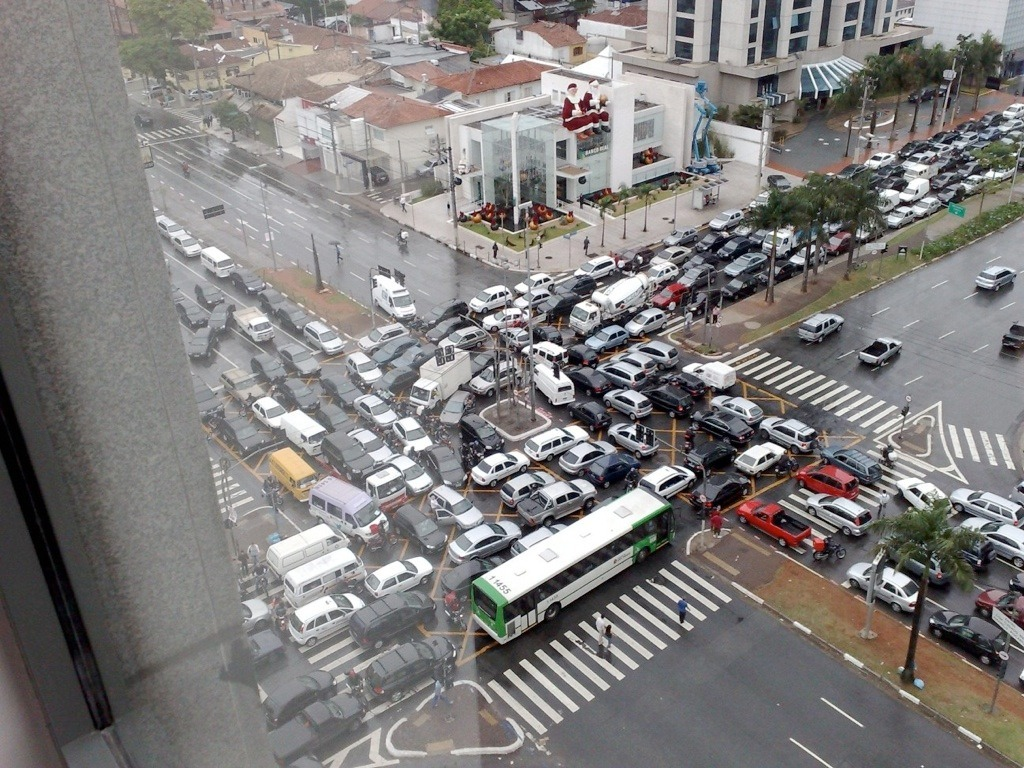
\includegraphics[width=.8\textwidth]{L10/traffic-disaster}
  \end{center}
\end{frame}

\begin{frame}
  \frametitle{Interrupts Complicate OS Synchronization}
  \begin{changemargin}{2cm}\small
    Reference: \\[1em]
    Lin Tan, Yuanyuan (YY) Zhou, Yoann Padioleau.\\
    ``aComment: Mining Annotations from Comments and Code to Detect Interrupt-Related Concurrency Bugs.''\\
  International Conference on Software Engineering, 2011.
  \end{changemargin}
\end{frame}

\begin{frame}
  \frametitle{Interrupts Complicate OS Synchronization}
  \begin{center}
    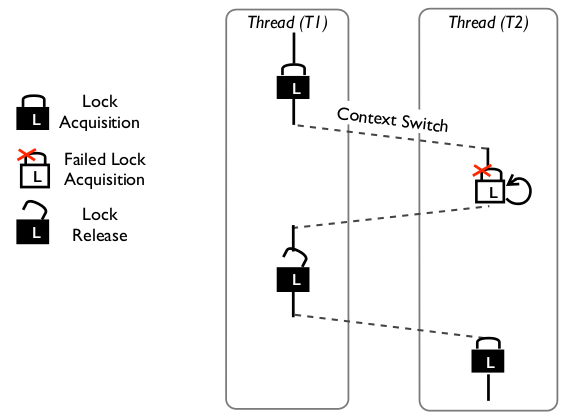
\includegraphics[width=.8\textwidth]{L10/lock-acq1}
  \end{center}
\end{frame}

\begin{frame}
  \frametitle{Interrupts Complicate OS Synchronization}
  \begin{center}
    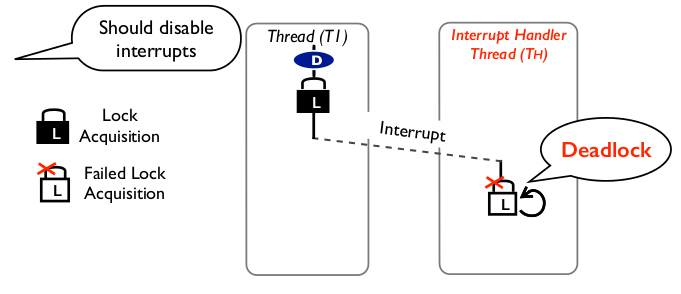
\includegraphics[width=.8\textwidth]{L10/lock-acq2}
  \end{center}
  \begin{changemargin}{0.5cm}
    If: spinlock taken by code that runs in interrupt context (hw or sw).\\
    Then: must use spin\_lock form that disables interrupts.\\
    Otherwise: sooner or later, you'll deadlock. 
\includegraphics[height=1em]{L10/look_of_disapproval}
  \end{changemargin}
\end{frame}

\begin{frame}[fragile]
  \frametitle{Disabling interrupts: spin\_lock\_irqsave}
  \begin{lstlisting}
    spinlock_t mr_lock = SPIN_LOCK_UNLOCKED;
    unsigned long flags;
    spin_lock_irqsave(&mr_lock, flags);
    /* critical section... */
    spin_lock_irqrestore(&mr_lock, flags);
  \end{lstlisting}

  \begin{changemargin}{2cm}
    {\tt spin\_lock\_irqsave()} disables interrupts locally and provides spinlock on symmetric multiprocessors (SMPs).\\[1em]
    {\tt spin\_lock\_irqrestore()} restores interrupts to state when lock acquired.\\[1em]

    This covers both interrupt and SMP concurrency issues.\\[1em]
  \end{changemargin}
\end{frame}

\end{document}
